\documentclass[12pt,a4paper]{article}

\usepackage[letterpaper]{geometry}
\usepackage{times}
\geometry{top=1.0in, bottom=1.0in, left=1.0in, right=1.0in}


\usepackage{fancyhdr}
\pagestyle{fancy}
\lhead{} 
\rhead{}
\chead{} 
\lfoot{} 
\cfoot{} 
\rfoot{} 
\renewcommand{\headrulewidth}{0pt} 
\renewcommand{\footrulewidth}{0pt} 
%To make sure we actually have header 0.5in away from top edge
%12pt is one-sixth of an inch. Subtract this from 0.5in to get headsep value
\setlength\headsep{0.333in}

\usepackage{fontspec}
\setmainfont{Times New Roman}

\usepackage{graphicx}



% =============================
\begin{document}

\linespread{2}

% =============================

%NOTE: cover page
\begin{center}
\vspace*{0.7in}
%\includegraphics[width=0.55\textwidth]{./pot}\\[1cm]    
\vspace*{0.7in}

%\textsc{\Large Major Research Paper}\\[0.5cm]


% Title


% Author and supervisor

\begin{center} 


\includegraphics[height=3cm]{picture/umjiLogo}


{
\linespread{2}
\LARGE
\textsc{VG100 Introduction To Engineering} \\
}
{
\Large
\textsc{Project 1 Bridge Crane} \\
}


\vspace*{0.6in}

\textsc{\large Group 3 Trinity}\\

\vspace*{0.2in}


\begin{tabular}{cc}
{\fontspec{Hei}\selectfont 谢舒翔} & Shuxiang \textsc{Xie} \\
{\fontspec{Hei}\selectfont 郭成彰} & Chengzhang \textsc{Guo} \\
{\fontspec{Hei}\selectfont 麻珂睿} & Kerui \textsc{Ma} \\
{\fontspec{Hei}\selectfont 王韧} & Ren \textsc{Wang} \\
{\fontspec{Hei}\selectfont 朱波颖} & Boying \textsc{Zhu} \\
\end{tabular}


\vspace*{0.5in}

\begin{tabular}{cc}
Professor & Yanfeng \textsc{Shen} \\
Professor & Cynthia \textsc{Vagnetti} 
\end{tabular}


\vspace*{0.7in}

{\today}


\end{center}



% Bottom of the page
\end{center}
\newpage
% NOTE: end of cover page

% =============================

\rhead{\textsc{Group 3}}
\lhead{
\includegraphics[height=1cm]{picture/umjiLogo}}

\tableofcontents
\newpage

\section{Introduction}

\subsection{About Us and Campus}


\begin{figure}[htbp]
\centering

\includegraphics[height=8cm]{picture/teamMember}
  \caption{Our team \label{fig:teamMember}}
\end{figure}

We are TRINITY (Figure \ref{fig:teamMember}), a team of freshmen from University of
Michigan-Shanghai Jiao Tong University Joint Institute (UM-SJTU JI), which is
located in the campus of Shanghai Jiao Tong University (Figure
\ref{fig:campus}). People in the photo are Xie Shuxiang, Zhu Boying, Ma Kerui,
Wang Ren and Guo Chengzhang, and our group leader is Xie Shuxiang. Joint
Institute is well-known for its unique way of helping students develop the
ability of cooperation and innovation. As a result, students here have various
projects and activities to attend to broaden their horizons.  


\begin{figure}[htbp]
\centering
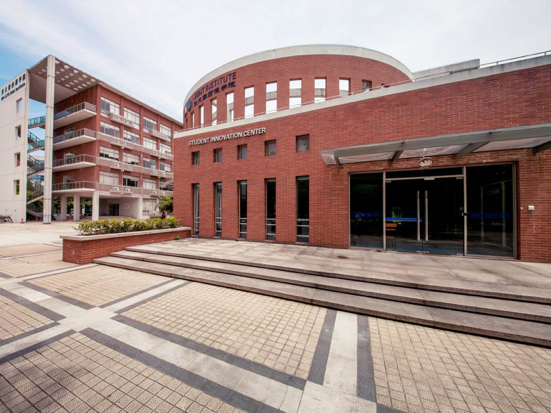
\includegraphics[height=5cm]{figure/campus}
  \caption{\label{fig:campus}}
\end{figure}

\subsection{Course and Project Information}


VG100 is a course about Introduction to Engineering. It is a mandatory course
for all freshmen in JI. According to Professor Shen Yanfeng, the course not only
convey fundamental knowledge of engineering, but also help students learn how to
solve a realistic problem. Besides, the technical communication part strengthens
students’ ability of taking part in teamwork, which is of great importance for
engineers.  

The first project students should accomplish in VG100 is to make a bridge-crane
system. It should be able to allow a cart to pull a cup of water up, travel
forward on the bridge to the other side, and put down the cup of water on the
designated place (Figure \ref{fig:structureOfP1}).  

\begin{figure}[htbp]
\centering
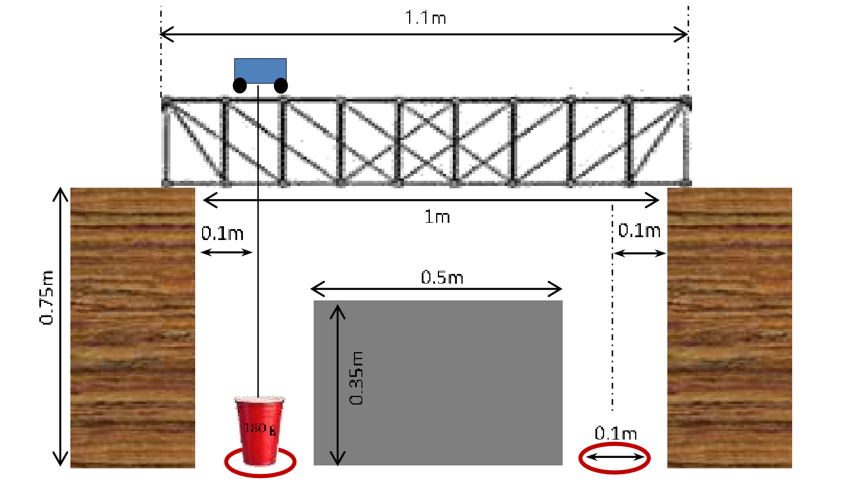
\includegraphics[height=5cm]{figure/structureOfP1}
\caption{\label{fig:structureOfP1}}
\end{figure}

The following list from the professor shows the specific requirement of Project 1.
Mechanism: Any method that can achieve the above task will be acceptable.
Breaking any of these rules will result in failing project 1.  
Bridge length:  >= 1.1m 
Bridge width:  <= 0.2 m 
Bridge Material: printing paper (80g size A4) and non-toxic, white wood glue
(brand: LongMa). Any additional material violates the rule!  
Maximum Mass of the bridge: 200g 
Maximum length of the cart: 0.1 m 
Power Supply: Maximum two portable Power Supply (for each battery Voltage ≤ 12V) 
Motor specifications: < 12V.  
Central Control Circuit: Arduino series (Required for Programming \& Can Be Omitted)

\subsection{Race Performance}
(This part will be completed later)

 % introduction
\section{Design Overview}
\subsection{Bridge}
This bridge has a limited weight and length. The weight of the bridge needs to
bear is more than 500 grams. To reach this goal, we need a proper structure and
craftsmanship. More details and limitations will be discussed as follows: 

\bigskip
\noindent
\textbf{Materials} \\
\indent
There are two kinds of materials: while glues and A4 paper.
While glue's brand is LongMa, and the A4 paper’s type is 80$g/m^2$.

\bigskip
\noindent
\textbf{Design concept} \\
\indent
Because the cart will lay down a rope to raise the cup of water up, it’s
impossible to set beams between the two sides’ bridge. We decide to take truss
structure to add its bearing load and its stability.

 
\bigskip
\noindent
{\large\textbf{Components Design}} \\
\textbf{Beam design} \\
\indent
At beginning, we tried the cube beam to make sure the beams can be placed in a
stable condition on the table. However, this design needs 4 layers of paper to
form one beam, because of square’s instability. By calculating the bending
stress and consulting the professor, we decided to use cuboid cube beams to
achieve a lighter weight, whose cross section is $5mm\times10mm$. 


\bigskip
\noindent
\textbf{Structure design} \\
\indent
This part includes connection and the structure. We connected two truss
structures as two sides of the bridge. On each side, we added three short beams
below the main beam and paste long paper script between beams to bear and
disperse the force generated by the cart (more detail and structure picture can
be found in the next part.) 

\bigskip
\noindent
\textbf{Design Visualization:} \\
\indent

%TODO: add pictures



\subsection{Cart}

The cart has ten main parts to fulfill the requirements: base, servo, wheel,
motor, battery, Arduino Board, Motor Driver and voltage transformer.

\bigskip
\noindent
\textbf{Base: Carbon Fibre} \\
\indent
Although we considered using Acrylic board, the fact that it is too thick, too
heavy and easy to break make us decide to use carbon fibre.
Carbon fibre is much lighter and stronger.
It also has a better looking. 

\bigskip
\noindent
\textbf{Servo: MG996R}  \\
\indent
We decided to use servo instead of motor to lift water because servo is more
powerful and easy to assemble. 
The first type we used is P0090.
It was not powerful enough, so we finally choose MG996R. 

\bigskip
\noindent
\textbf{Wheel: 3D-printed Plastic Wheel } \\
\indent
In order to fit the bridge, and meanwhile lower the influence to other parts of
the cart, we decided to print our own wheels in 3D.
The specially made wheels match the bridge well and guide the cart’s direction.

\bigskip
\noindent
\textbf{Motor: Gear motor N20 } \\
\indent
At first, we believe the high speed motor like 130 and 180 would give our cart
extraordinary speed.
But they were not powerful enough to move the cart on the bridge.
Also, the high speed motor has difficulty while stopping.
So we finally choose N20 gear motor.
It becomes slower but more powerful and stable.
In addition, N20 is also lighter than any high speed motor.  

\bigskip
\noindent
\textbf{Battery: 11.1V Battery } \\
\indent
The battery we chose has voltage 11.1V, which can well charge the Arduino board,
the motor board and the servo.
We choose 11.1V because we can have more choices of voltage using transformer.
We can adjust the speed of motor and servo easily.  

\bigskip
\noindent
\textbf{Arduino Board: UNO } \\
\indent
We first used Arduino UNO which was very light and small; however, we found it
too unreliable and not proper enough to be assemble on the cart, so we changed
to Arduino UNO.
It can provide all the functions we need stalely with a little weight increase.

\bigskip
\noindent
\textbf{Motor Driver: Motor Driver L9110 } \\
\indent
We first used Motor Driver L298n, which was provided by our project instructor;
however, we found the cooling n too heavy and to a certain degree useless for
our low-power cart, so we changed to Motor Driver L9110.

\bigskip
\noindent
\textbf{Voltage transformer:} \\
\indent
First, we did not use transformer to power the servo but Arduino board.
It takes more than 5 seconds to pull up the water.
After taking some calculation, the increase in voltage will shorten the time to
70\%.
So we finally applied transformer and lower the 11.1V from battery to 7.4V to
power the servo.

\subsection{Overall} % design over view
\section{Materials \& Tools}
% images
\newcommand{\beginMyTabular}{
    \begin{center}
    \begin{tabular}{p{0.4cm}p{5cm}p{5cm}rr}
    \hline
    No. & Item & Specification & Quantity & Price(Yuan) \\
    \hline
}
\newcommand{\MyTabularEnd}{
    \hline
    \end{tabular}
    \end{center}
}
% counter
\newcounter{matcnt}
\setcounter{matcnt}{0}
\newcommand{\CounterOfM}{
    \stepcounter{matcnt}\arabic{matcnt}
}
% CounterOfM means the counter of materials
%
\newcounter{figcnt}
\setcounter{figcnt}{0}
\newcommand{\CounterOfF}{
    \stepcounter{figcnt}\arabic{figcnt}
}
\newcommand{\CounterOfFa}[1]{
    \raisebox{#1cm}{
        \fbox{\small \CounterOfF} \hspace{0.3cm}
    }
    \nolinebreak[3]
}
\newcommand{\MPGx}[3]{
    \CounterOfFa{#1}
	\begin{minipage}{0.2\textwidth}
    \centering    
    \includegraphics[height=#2cm]{picture/material/#3}
    \end{minipage}
}
\newcommand{\MPGxA}[3]{
    \CounterOfFa{#1}
	\begin{minipage}{0.1\textwidth}
    \centering    
    \includegraphics[height=#2cm]{picture/material/#3}
    \end{minipage}
}
%% ====================================================
%% ====================================================
%% ====================================================
\newcommand{\HPRx}{1.4}
\newcommand{\HPx}{2}
\newcommand{\MyWidthFirstLine}{3.3cm}

%\begin{flushleft}
%\begin{tabular}{p{\MyWidthFirstLine}p{\MyWidthFirstLine}p{\MyWidthFirstLine}p{\MyWidthFirstLine}}
%\end{tabular}
%\end{flushleft}
%
\begin{center}
\begin{tabular}{lll}
\MPGxA{\HPRx}{\HPx}{a4paper} & \MPGxA{\HPRx}{\HPx}{whiteglue} & \MPGxA{\HPRx}{\HPx}{papercutter} \\
\MPGxA{\HPRx}{\HPx}{brush} & \MPGx{\HPRx}{\HPx}{woodstick} & \MPGx{\HPRx}{\HPx}{scissor} \\
\MPGx{\HPRx}{\HPx}{arduino} & \MPGx{\HPRx}{\HPx}{standN20} & \MPGx{\HPRx}{\HPx}{moterN20} \\
\MPGx{\HPRx}{\HPx}{wheelrubber} & \MPGx{\HPRx}{\HPx}{servo360} & \MPGx{\HPRx}{\HPx}{batteryPlane} \\
\MPGx{\HPRx}{\HPx}{batteryBreeze} & \MPGx{\HPRx}{\HPx}{switch} & \MPGx{\HPRx}{\HPx}{pcbBoard} \\  
\MPGx{\HPRx}{\HPx}{tapeThick} & \MPGx{\HPRx}{\HPx}{stringYoYo} & \MPGx{\HPRx}{\HPx}{m3} \\ 
\MPGx{\HPRx}{\HPx}{m2} & \MPGx{\HPRx}{\HPx}{car} \\
\end{tabular}
%
\end{center}
%
\subsection{Bridge}
\subsubsection{Materials}
% tables
\beginMyTabular
\CounterOfM & A4 paper & Double A 80 g  A4 paper  & 10 & 29.8 \\
\CounterOfM & Long Ma White Glue & 400 g & 5 & 67.5 \\
\MyTabularEnd

\subsubsection{Tools}

% images

% tables
\beginMyTabular
\CounterOfM & Huanmei Paper Cutter & & 1 & 34.8 \\
\CounterOfM & Brush & 5 mm width & 5 & 10.6 \\
\CounterOfM & Wood Stick & 5 mm $\times $ 5 mm & 10 & 4 \\ 
\CounterOfM & Qixing Scissor &  & 1 & 4.6 \\ 
\MyTabularEnd

% ======================================

\subsection{Cart}
\subsubsection{Materials}

% tables
\beginMyTabular
\CounterOfM & XTWduino UNO Arduino & V3.0 ATMEGA328P & 1 & 25\\
\CounterOfM & N20 stand &  & 1 & 0.99\\
\CounterOfM & N20 Moter & 12V 150 rpm & 1 & 19.80 \\
\CounterOfM & Rubber Wheel & Diameter: 43 mm  &  2  & 5.4 \\
\CounterOfM & TowerPro 360 Degree servo & MG996R  & 1 & 38\\
\CounterOfM & Plane model Battery & 7.4 &1  & 37.8\\
\CounterOfM & Breeze 2s/3s Battery & 11.1V 500mAh& 1& 31\\
\CounterOfM & Bridge-shaped  Switch & &1 &1.6 \\
\CounterOfM & PCB Hole Board & 9 * 15 cm Gap 2.54 mm & 1 & 6 \\
\CounterOfM & 3M Thick Plastic tape & 1 cm Width & 1 & 7 \\
\CounterOfM & Audi YoYo String & & 1 & 7.9 \\
\MyTabularEnd

\subsubsection{Tools}
% images

% tables
\beginMyTabular
\CounterOfM & M3 screws and nuts  & 3 mm & 2 & 0.75 \\
\CounterOfM & M2 screws and nuts & 2 mm &  4 & 0.65  \\
\CounterOfM & Model cart &  & 1 & 28 \\
\MyTabularEnd % material
\section{Improvements} % improvement
\section{Reference} % reference

\end{document}